\chapter{End of chapter exercise solutions}
\label{eoceSolutions}



%_______________
\eocesolch{Introduction to data}



%_______________
\begin{multicols}{2}

% 1

\eocesol{(a)~Possible answers: $^1$Basically true. Categorical variables have no numerical meaning. Examples: Hair color, gender, field of study. $^2$As a kind of counterexample, consider something like \emph{What is your favorite number among $\sqrt 2$, $\sqrt{-1}$, and $\pi$?}
Here it doesn't make much sense to take the average of the responses, so it is not your typical numerical variable. But it does involve numbers.\\
(b)~Possible answers: $^1$Basically true. A discrete variable is a variable whose value is obtained by counting; a continuous variable is a variable whose value is obtained by measuring. %Thanks to Hau Nguyen.
$^2$As a kind of counterexample, consider a \emph{hybrid} variable $X$ which has a 50\% chance of $X=3$, and a 50\% of being a number $1\le X\le 2$, uniformly distributed (so that, given that $1\le X\le 2$, the probability that $X\le 5/4$ is 25\%, for instance).
(c)~Possible answers: $^1$Basically false. $^2$As a kind of counterexample, consider \emph{What is your favorite real number?} (where all real numbers are considered legitimate answers).
%\footnote{This is a solution to Exercise \ref{catcat}.}
}
% 3

\eocesol{(a)~New mean = 10+old mean $=70.7+10=80.7$.
(b)~New mean = $2\cdot$old mean $=70.7\cdot 2=141.4$. In formulae, $E(2X)=2E(X)=2(70.7)=141.4$ where $E(X)$ is the mean of $X$.
(c)~The means are
\begin{eqnarray*}
	&=&\frac{x_1+c_1+x_2+c_1+\dots+x_n+c_1}n\\
	&=&\frac{nc_1+ (x_1+\dots+x_n)}n=c_1+\frac{x_1+\dots+x_n}n.
\end{eqnarray*}
and $\frac{x_1c_2+\dots+x_nc_2}n=c_2\frac{x_1+\dots+x_n}n$, respectively.
In formulae, $E(X+c_1)=E(X)+c_1$ and $E(c_2X)=c_2E(X)$.
%\footnote{This is a solution to Exercise \ref{extra_mean}.}
\footnote{By the way, a solution to 1.2 is mean $=(55+59+64+68+70+70+71+76+76+98)/10$=70.7, median = (70+70)/2=70, mode = 70,76.}
}

\eocesol{This uses Jensen's Inequality, which says that if $f''(x)\ge 0$ for all $x$ (so $f$ is \emph{concave up} or \emph{convex}) then a chord drawn between two points on the graph of $f$ will lie above the graph of $f$. In symbols, $f(tx_1+(1-t)x_2)\le tf(x_1)+(1-t)f(x_2)$ for al l$0\le t\le 1$. By iterating, we get for $a+b+c=1$,
\begin{eqnarray*}
	&&f(ax+by+cz)\\
	&=&f\left(ax+(1-a)\left(\frac{b}{1-a}y + \frac{c}{1-a}z\right)\right)\\
	&\le&af(x)+(1-a)f\left(\frac{b}{1-a}y + \frac{c}{1-a}z\right)\\
	&\le&af(x)+(1-a)\left(\frac{b}{1-a}f(y) + \frac{c}{1-a}f(z)\right)\\
	&=&af(x)+bf(y)+cf(z)
\end{eqnarray*}
and similarly for $a_1+\dots+a_n=1$, $f(\sum a_ix_i)\le\sum a_if(x_i)$.
In particular, since the function $f(x)=-\ln x$ satisfies $f''(x)=1/x^2\ge 0$ in its domain $x> 0$, and taking each $a_i=1/n$, we have
\[
	-\ln(\overline x) \le \overline{-\ln x} := \frac1n \sum -\ln x_i,
\]
which gives the arithmetic-geometric inequality by raising $e$ to the power of both sides. For the harmonic inequality, consider instead
\[
	n/\sum(1/x_i)=\left(\sum (1/x_i)/n\right)^{-1}
\]
which reduces the problem to the arithmetic-geometric inequality with $x_i$ replaced by $1/x_i$.
%\footnote{This is a solution to Exercise \ref{harmonic}.}
}

\eocesol{(a)~Let $g(x)=f(x)+c$. Then
\begin{eqnarray*}
	\mathrm{avg}_{g}&=& \frac1{b-a}\int_a^b g(x)\,dx\\
	&=& \frac1{b-a}\int_a^b f(x)+c\,dx = \mathrm{avg}_f + c.
\end{eqnarray*}
(b)~Let $h(x)=c\cdot f(x)$. Then
\begin{eqnarray*}
	\mathrm{avg}_h &=& \frac1{b-a}\int_a^b h(x)\,dx\\
	&=& \frac1{b-a}\int_a^b c\cdot f(x)\,dx = c\cdot\mathrm{avg}_g.
\end{eqnarray*}
%\footnote{This is a solution to Exercise \ref{inv_ave}.}
\footnote{By the way, a solution to 1.8 is:
Since $f$ is continuous, then there exists some number $c$ such that $a<c<b$, and
\[
f'(c)=\frac{f(b)-f(a)}{b-a}=\frac{\int_a^b f'(x)\,dx}{b-a}.
\]
Let $g(x)=f'(x)$,then
\[
g(c)=\frac1{b-a}\int_a^b g(x)\,dx=\mathrm{avg}_g.
\]
}
}

\eocesol{We have $(\frac43)(\frac32)=2=2^{12/12}=2^{5/12}2^{7/12}$. The inequalities both follow from $2^{19}=524,288<531,441=3^{12}$.}
%_______________
\end{multicols}


%\textC{\newpage}


%_______________
\eocesolch{Probability}



%_______________
\begin{multicols}{2}

% 1

\eocesol{(a)~Use the substitution $u=(x-\mu)/\sigma$.
(b)~What we need to verify: for the mean, $\int x f(x)\,dx=\mu$ (use the substitution $u=x-\mu$ in the integral). For the median, $P(X\le\mu=1/2$. For the mode, $\varphi'(\mu)=0$.
(c)~The variance is $E(X^2)-E(X)^2$ so we need to evaluate $E(X^2)=\int x^2\varphi(x)\,dx$.
%\footnote{This is a solution to Exercise \ref{normal_dist}}
}

% 3


\eocesol{(a)~We have $\int f(x)\,dx=1$ using the derivative of $\arctan$.\\
(b)~The median and mode are both 0, by symmetry $f(x)=f(-x)$ and since $f'(x)\le 0$ if and only if $x\ge 0$.\\
(c)~Hint: the mean would be $\int xf(x)\,dx$ but this is similar to the harmonic series $\sum_n 1/n$. You can use the substitution $u=1+x^2$.\\ %Thanks to Hau
(d)~Since the mean does not exist, we cannot claim that sample averages $\overline x_n$ from this distribution will converge to the mean. (If the mean were $+\infty$ we could perhaps argue that sample averages would diverge to $+\infty$, but since $-\infty$ is equally plausible as a mean here, all we can expect is ``chaos'' in the behavior of $\overline x_n$.
%\footnote{This is a solution to Exercise \ref{cauchy_dist}.}
}

%\eocesol{5\% increase in value.}
%\eocesol{5\% increase in value.}



%_______________
\end{multicols}



\newpage


%_______________
\eocesolch{Distributions of random variables}


\begin{figure}
\centering
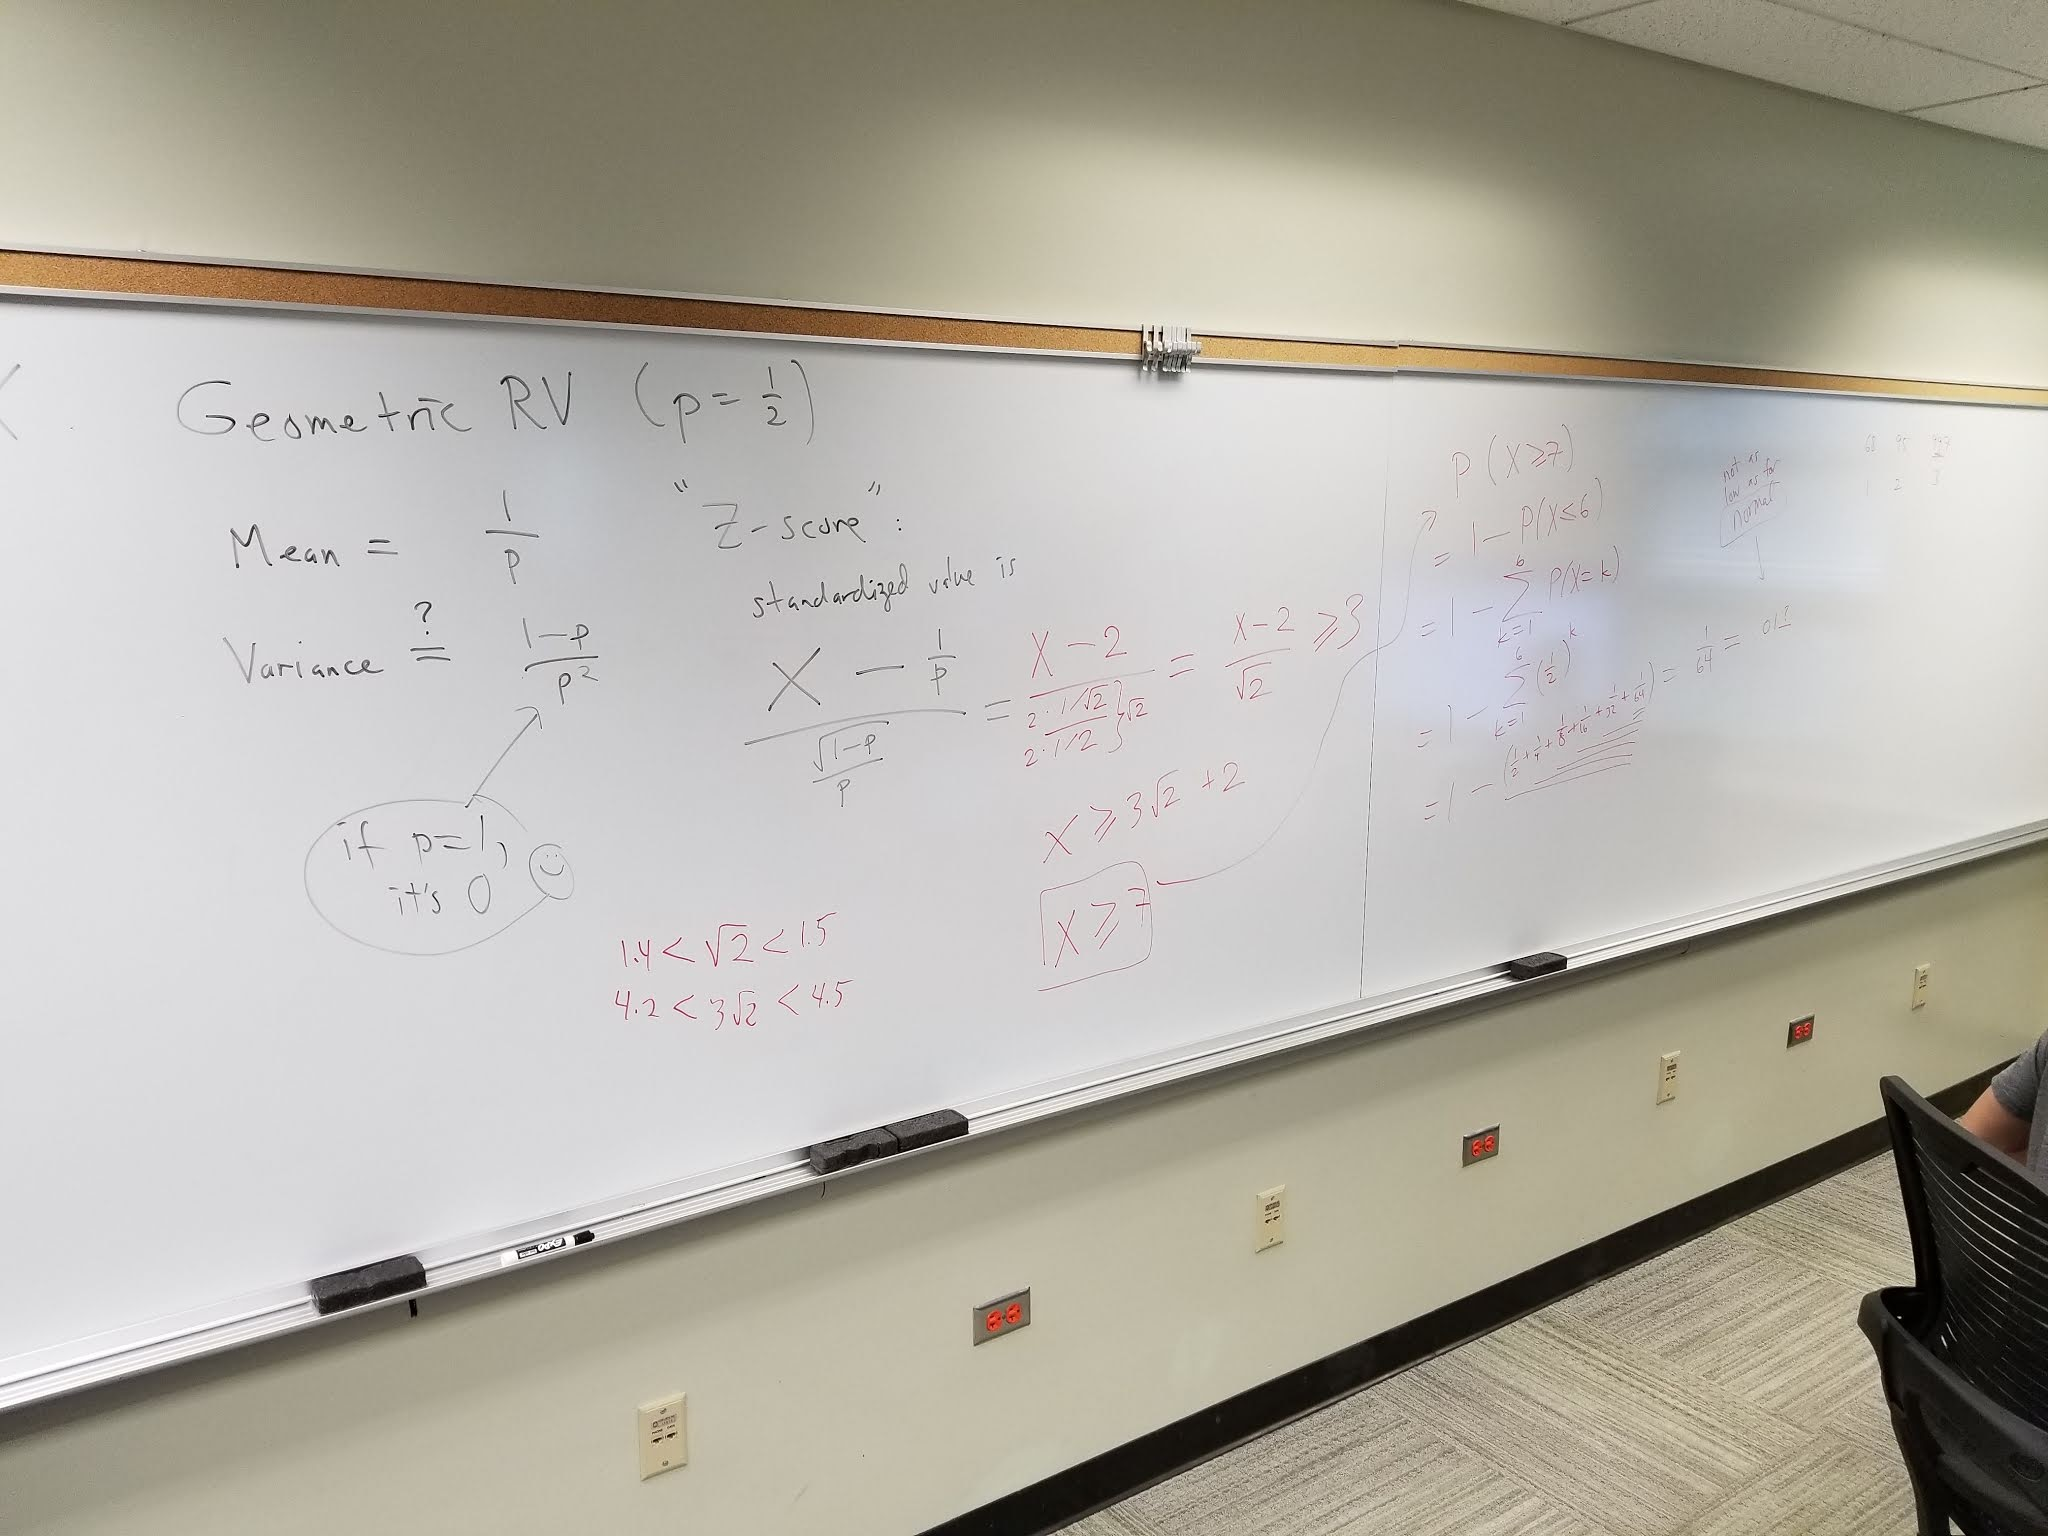
\includegraphics[width=5in]{extraTex/eoceSolutions/likelihoodprinciple}
\caption{A calculation related to the Likelihood Principle, from Fall 2018 in Webster Hall 101, UH M\=anoa campus.}\label{LP}
\end{figure}
%_______________
\begin{multicols}{2}

% 1

\eocesol{(a)~In general, normality is expected when dealing with variables for which the Central Limit Theorem holds approximately: sums of IID (independent, identically distributed) variables. A safe example is proportions of heads and tails when flipping a coin. Height of individuals may be an example if a person's height is approximately the result of a sum of independent events such as healthy meals, nights of sufficient sleep (for the individual or for their parents), etc.\\
(b)~This is a tricky one; a library deep-dive into the given article is probably your best bet.\\
(c)~We assume the student can look up things like \emph{power-law distribution} online. One example is then \emph{the frequencies of words in most languages}.
%\footnote{This is a solution to Exercise \ref{skewed_but_real}.}
\footnote{And here is a solution to 3.2 Three Sigma: (a)~$P(X=3)=0.5(1-0.5)3-1=0.125=12.5\%$; $P(X=10)=0.5(1-0.5)10-1=0.00097=0.097\%$; $P(X=100)=0.5(1-0.5)100-1=0\%$.
(b)~$P(Z>3)=1-P(Z<3)=1-0.99865=0.00135$, $\implies$0.5(1-0.5)n-1=0.00135, $\implies n\ge 9.5$. However, interestingly, if we consider the geometric distribution instead we get a different answer. This relates to a famous discussion about the Likelihood Principle \url{https://en.wikipedia.org/wiki/Likelihood_principle} (see Figure \ref{LP}).}
}{}

% 3

\eocesol{(a)~This is just $P(X=k-1)$ where $X$ is binomial with parameters $p$ and $n-1$. To wit:
\begin{eqnarray*}
	&&\binom{n-1}{k-1} p^{k-1}(1-p)^{(n-1)-(k-1)}\\
	&=& \binom{n-1}{k-1} p^{k-1}(1-p)^{n-k}.
\end{eqnarray*}
(b)~Since the $n$th trial is independent of the previous trials, this is
\begin{eqnarray*}
	&&p\cdot \binom{n-1}{k-1} p^{k-1}(1-p)^{n-k} \\
	&=&\binom{n-1}{k-1} p^{k}(1-p)^{n-k}.
\end{eqnarray*}
(c)~The answer to (b) is exactly the probability that a negative binomial variable $Y$ with parameters $n$ and $p$ will take value $k$.
This is not surprising since the following two conditions are equivalent:
\begin{itemize}
\item the first success happens in trial $n$;
\item the first $n-1$ trials are failures and the $n$th trial is a success.
\end{itemize}
%\footnote{This is a solution to Exercise \ref{negative_binomial}.}
}

% 5
\eocesol{We solve for $\beta$:
\[
\beta=\frac{x}{1-x}\left(2\alpha+\frac1{1-x}\right)
\]
Then
\begin{eqnarray*}
E(X^2)&=&\sum_{k=1}^\infty k^2 P(X=k)\\
&=&\sum_{k=1}^\infty k^2 (1-p)^{k-1}p = \frac{p}{1-p}\sum_{k=1}^\infty k^2 (1-p)^k\\
&=& \frac{p}{1-p}\beta\\
&=& \frac{p}{1-p} \frac{1-p}{p} \left(2\frac{1-p}{p^2} +\frac1p\right)\\
&=& \frac{2-2p+p}{p^2} = \frac{2-p}{p^2}
\end{eqnarray*}
giving $\sigma^2 = \frac{2-p}{p^2}-(1/p)^2 = \frac{1-p}{p^2}$, as desired.
}{}

\end{multicols}
%_______________
\eocesolch{Foundations for inference}



%_______________
\begin{multicols}{2}

% 1

\eocesol{(a)~If you are wondering whether a certain drug helps to cure cancer, you are not interested in proving that the drug just changes the outcomes for cancer.
You really want it to help and not hurt. So a 1-sided test is appropriate.\\
(b)~If you are hoping that a certain coin is fair, you don't necessarily care in which direction it may be biased.
Too many heads and too many tails are not different outcomes for you, in any interesting sense. So you want a 2-sided test.}

% 3
\eocesol{(a)~If $X$ and $Y$ are independent then so are any deterministic (not random) functions of them $f(X)$, $g(Y)$. 
Moreover, whenever $U$ and $V$ are independent then $E(UV)=E(U)E(V)$. These facts are proved in more advanced texts.
In particular, for any constant $t$, $e^{tX}$ and $e^{tY}$ are independent, and
\begin{eqnarray*}
	M_{X+Y}(t)&=&E(e^{t(X+Y)}) = E(e^{tX}e^{tY})\\
	 &=& E(e^{tX})E(e^{tY}) = M_X(t)M_Y(t).
\end{eqnarray*}
The other part is easier:
\[
	M_{cX}(t)=E(e^{t(cX)}) = E(e^{(ct)X}) = M_X(ct).
\]
(b)~The power series of $e^x$ is $\sum x^n/n!$. Now assuming that $E(\sum)=\sum(E)$ (proved in advanced real analysis texts),
\begin{eqnarray*}
	M_X(t)=E(e^{tX}) &=& E\left(\sum (tX)^n/n!\right)\\
	 &=& \sum E(X^n)t^n/n!
\end{eqnarray*}
(c)~We have
\[
	M^{(n)}_X(0)= \frac{d^n}{dt^n}M_X(t)\bigg|_{t=0}.
\]
We then use $d/dt\sum^{\infty} = \sum^{\infty}d/dt$ (proved in advanced real analysis texts), and
\[
	\frac{d^n}{dt^n}t^n\bigg|_{t=0}=n!
\]
to finish.}

% 5
\eocesol{%(a)~easy\\
%(b)~nice.\\
%(c)~nice.\\
(d)~Suppose they are all bounded by $b$.\\
(e)~We use the fact that the normal distribution with mean $\mu$ and variance $\sigma^2$ is the only distribution whose cumulants are $\mu,\sigma^2,0,0,0,\dots$.}

\eocesol{
Hint: solve $90\%^k < 50\%$ for $k$.
}
\end{multicols}


\newpage

\eocesolch{Inference for numerical data}

%%%%%%%%%%%%%%%%%%%%%%%%%%%%%

\begin{multicols}{2}

% 1
\eocesol{The price of \emph{Statistics for Calculus Students} printed and bound, in the UCLA bookstore and on Amazon, is an example of paired data. The price of \emph{Stats: Data and Models} by de Veaux, at UCLA, and \emph{Probability: theory and examples} by Durrett, on Amazon, is an example of unpaired data.}

\eocesol{(a)~We are selecting a substantial proportion of the homes. Let's say we look at the proportion who plan to vote for the Democratic candidate (or, alternatively, the Republican candidate). If the sample was small compared to the population, but still large in absolute terms, we could argue that we have a sampling distribution to which the Central Limit Theorem applies. But 20\% is too large a sample, creating dependencies. For instance, if all of the first 10\% vote Republican it becomes unlikely that many of the other 10\% vote Democrat. \\
(b)~Now the proportion of homes selected is small enough for most purposes. However, the sample size of 10 is a bit small for the normal approximation to be reliable.}

% 3
\end{multicols}
% Chp 6
\eocesolch{Inference for categorical data}

%%%%%%%%%%%%%%%%%%%%%%%%%%%%%

\begin{multicols}{2}

% 1
\eocesol{(a)~A hint is already given.\\
(b)~We have
\[
	\Gamma(1/2) = \int_0^\infty t^{1/2-1} e^{-t}\,dt = \int_0^\infty \frac{dt}{e^t\sqrt{t}}.
\]
Now try the substitution $t=u^2/2$.}

\eocesol{Note that there are some ``easy'' solutions that don't quite work. But moment generating functions can be used:
\[
	M_{X_1+X_2}(t) = M_{X_1}(t) M_{X_2}(t)
\]
Solve for $M_{X_2}(t)$.}

% 3
\eocesol{Squaring both sides, %\begin{eqnarray*}
%	\sqrt{(\hat p_y(1-\hat p_y)/1924)+(\hat p_x(1-\hat p_x)/3666)} &=& 0.01\\
%	\hat p_y-\hat p_x&=&0.04
%\end{eqnarray*}
\begin{eqnarray*}
	\frac{\hat p_y(1-\hat p_y)}{1924}+\frac{\hat p_x(1-\hat p_x)}{3666} &=& 10^{-4}\\
	\hat p_y-\hat p_x&=&\frac1{25}
\end{eqnarray*}
\begin{eqnarray*}
	\frac{(\hat p_x+\frac1{25})(1-\hat p_x-\frac1{25})}{1924}+\frac{\hat p_x(1-\hat p_x)}{3666} &=& 10^{-4}
\end{eqnarray*}
\[
	\frac{(u+\frac1{25})(1-u-\frac1{25})}{1924}+\frac{u(1-u)}{3666} = 10^{-4}
\]
This we can solve by hand; Wolfram Alpha gives\footnote{\url{https://www.wolframalpha.com/input/?i=\%5Cfrac\%7B(u\%2B\%5Cfrac1\%7B25\%7D)(1-u-\%5Cfrac1\%7B25\%7D)\%7D\%7B1924\%7D\%2B\%5Cfrac\%7Bu(1-u)\%7D\%7B3666\%7D+\%3D+10\%5E\%7B-4\%7D}}
$u = 5093/10750 - \sqrt{7133687/2}/5375$, i.e., $u\approx 0.12240$ or $u\approx 0.82514$.
Looking at the paper \footnote{\url{http://thegeeksverse.com/wp-content/uploads/2014/09/SexOrColorPref.pdf}}, we see that actually
$p_y=233/1924=.1211$ and $p_x=306/3666=.0835$ which gives the standard error $0.0087\approx 0.01$.
%\footnote{This is a solution to Exercise \ref{zain_email}.}
}

\end{multicols}

\newpage

\eocesolch{Introduction to linear regression}

\begin{multicols}{2}

% 1
\eocesol{(a)~The points $\{(0,0),(1,1),(2,2)\}$ form one example. We need at least 3 points for $r$ to be defined because of the $n-2$ in a denominator.\\
(b)~Using
\[
r =\frac{\sum ^n _{i=1}(x_i - \bar{x})(y_i - \bar{y})}{\sqrt{\sum ^n _{i=1}(x_i - \bar{x})^2} \sqrt{\sum ^n _{i=1}(y_i - \bar{y})^2}}
\]
When $n=0$ or $n=1$, we have all $x_i=\bar{x}$ and $y_i=\bar{y}$, hence $r$ is of the form ``$0/0$'' and undefined.
When $n=2$, $x_1-\bar{x}=x_1-\frac{x_1+x_2}2 = \frac{x_1-x_2}2$ and
\begin{eqnarray*}
r &=&\frac{\frac{x_1 - x_2}2 \frac{y_1-y_2}2 + \frac{x_2-x_1}2\frac{y_2-y_1}2}{\sqrt{2((x_1-x_2)/2)^2 2((y_1-y_2)/2)^2}}\\
&=&\frac{\frac{x_1 - x_2}2 \frac{y_1-y_2}2 + \frac{x_2-x_1}2\frac{y_2-y_1}2}{2\sqrt{((x_1-x_2)/2)^2 ((y_1-y_2)/2)^2}}\\
&=&2\frac{\frac{x_1 - x_2}2 \frac{y_1-y_2}2 + \frac{x_2-x_1}2\frac{y_2-y_1}2}{\sqrt{((x_1-x_2))^2 ((y_1-y_2))^2}}\\
&=&\frac{(x_1-x_2)(y_1-y_2)}{\abs{(x_1-x_2)(y_1-y_2)}}\\
&=&\mathrm{sign}((x_1-x_2)(y_1-y_2)),
\end{eqnarray*}
where
\[
\mathrm{sign}(x)=
\begin{cases}
1& \text{if }x>0,\\
-1&\text{if }x<0,\\
\text{undefined}&\text{if }x=0.
\end{cases}
\]
In any case, this is a long-winded way of saying that there can be no example with $n=2$, either.
How about $n=3$? We get the algebraic equation
\begin{eqnarray*}
&&   (2x_1-x_2-x_3)(2y_1-y_2-y_3)\\
&+& (2x_2-x_3-x_1)(2y_2-y_3-y_1)\\
&+& (2x_3-x_1-x_2)(2y_3-y_1-y_2) = 0.
\end{eqnarray*}
with the constraint that not all $x_i=\bar x$, and not all $y_i=\bar y$.\footnote{It may be tempting to propose $\{(0,0), (1,0), (2,0)\}$ as an example of $r=0$, based on the idea that when the slope is 0, there is no positive or negative correlation, so the correlation is 0. But technically, that is incorrect, as $r$ will be undefined when there is no variation in the $y$-values. What is correct is that $b_1=0$ for this example.}%Thanks to Ethan Lamb for this example.
We might as well assume $(x_3,y_3)=(0,0)$, which gives
\begin{eqnarray*}
&&   (2x_1-x_2)(2y_1-y_2)\\
&+& (2x_2-x_1)(2y_2-y_1)\\
&+& (-x_1-x_2)(-y_1-y_2) = 0.
\end{eqnarray*}
If we also assume $(x_2,y_2)=(1,1)$, this becomes
\begin{eqnarray*}
&&   (2x_1-1)(2y_1-1)\\
&+& (2-x_1)(2-y_1)\\
&+& (x_1+1)(y_1+1) = 0.
\end{eqnarray*}
Let us rewrite it in variables without subscripts:
\[
   (2x-1)(2y-1)+ (2-x)(2-y)+ (x+1)(y+1) = 0.
\]
This simplifies (Wolfram Alpha) to $(2 x - 1) y = x - 2$.
So we can take $x=-1$ and $y=1$.\\
(c)~This is similar to (a). Take $\{(0,0), (1,-1), (2,-2)\}$ for instance.
\footnote{Here is a solution to 7.2 (Cauchy-Schwarz):
(a)
Expanding the terms
\[
(u_1x+v_1)^2+\dots+(u_nx+v_n)^2 
\]
Yields
\[
u_1^2x^2+2u_1v_1x+v_1^2+\dots+u_n^2x^2+2u_nv_nx+v_n^2
\]
Factoring common powers of x gives
\[
(u_1^2+\dots+u_n^2)x^2+(2u_1v_1+\dots+2u_nv_n)x+(v_1^2+\dots+v_n^2)
\]
(b)
The discriminant $D$ tells us
\begin{itemize}
\item there are two real roots if $D>0$;
\item there is a real root if $D\ge 0$;
\item there are no real roots if $D<0$.
\end{itemize}
The polynomial has at most most one root, therefore the discriminant is less than or equal to 0.
So since $D=b^2-4ac$,
\[
(2u_1v_1+...+2u_nv_n)^2-4(u_1^2+...+u_n^2)(v_1^2+...+v_n^2)\le 0,
\]
\[
4(u_1v_1+...+u_nv_n)^2\le 4(u_1^2+...+u_n^2)(v_1^2+...+v_n^2),
\]
\[
(u_1v_1+...+u_nv_n)^2\le (u_1^2+...+u_n^2)(v_1^2+...+v_n^2),
\]
as desired.}
}

% 3
\eocesol{(a)~Square both sides, multiply through to clear denominators, and use your algebra.
}{}

% 45

\end{multicols}





\eocesolch{Hidden Markov models}

\begin{multicols}{2}

% 1
\eocesol{(a)~The probability that $X=1$ and $Y=0$, for instance, is the probability that $X=1$, minus the probability that $X=1$ and $Y=1$.}

\eocesol{(a)~Here we have to consider the equation $p(1-p)n=\sigma^2$ and replace occurrences of $p$ by expressions involving $\sigma$.
}

\eocesol{Here is a solution to 8.2(a). 
$\mu=np$ and $p=\mu/n$. So $P(X=i)=\binom{n}{i} p^i (1-p)^{n-i}$ and $L(\mu)=\binom{n}{i}(\mu/n)^i(1-\mu/n)^{n-i}$.
(b)~Let $x_1,\dots,x_m$ be a random sample. Then starting with $L(\vec x,\mu)$ and taking logs, and differentiating with respect to $\mu$, and setting it equal to 0, we get $\mu=\sum_{i=1}^m x_i/m$, which is not surprising
as that is our sample mean.
}
% 3
%\eocesol{(a)~$\widehat{baby\_\hspace{0.3mm}weight} = -80.41 + 0.44 \times gestation - 3.33 \times parity - 0.01 \times age + 1.15 \times height + 0.05 \times weight - 8.40 \times smoke$.
%(b)~$\beta_{gestation}$: The model predicts a 0.44 ounce increase in the birth weight of the baby for each additional day of pregnancy, all else held constant.  $\beta_{age}$: The model predicts a 0.01 ounce decrease in the birth weight of the baby for each additional year in mother's age, all else held constant. 
%(c)~Parity might be correlated with one of the other variables in the model, which complicates model estimation.
%(d)~$\widehat{baby\_\hspace{0.3mm}weight} = 120.58$.
%$e = 120 - 120.58 = -0.58$. The model over-predicts this baby's birth weight.
%(e)~$R^2 = 0.2504$. $R_{adj}^2 = 0.2468$.}

\eocesol{%Zain's solution to Functional Margin
Given 
\[
\gamma_i = \frac{(\bar{w^T}\bar{x}+b)}{\|(wTx+b)\|}
\]
\[
\bar{w^T}\bar{x}-b=0\implies \bar{w^T}\bar{x}=b\implies (\bar{w^T}\bar{x})^2-b^2=0
\]
\[
\gamma_i\cdot(\text{Line})=\gamma_i\cdot (w^Tx-b)=0.
\]
Therefore the two are perpendicular because the dot product is zero.%\footnote{This is a solution to Functional Margin.}

}{}
\end{multicols}
